\documentclass[12pt]{article}[A4]
\usepackage[utf8]{inputenc}
\usepackage[spanish,es-tabla]{babel}
\usepackage{amsmath,multicol}

%\usepackage[resetlabels,labeled]{multibib}
%\usepackage[sorting=none, style = ieee]{biblatex}
\usepackage{cite}
%\addbibresource{sections/bib.tex}

\usepackage{fancyhdr}
\usepackage{import}
\usepackage{tikz}
\usepackage{booktabs}
\usepackage{graphicx,float,subcaption}
\newcommand{\gr}{^{\circ}}
\newcommand{\ohm}{\Omega}
\usepackage{import}
\usepackage{wrapfig}
\usepackage{url}
\usepackage{color}
\usepackage{epsfig}
\usepackage{booktabs}
\usepackage{multirow}
\usepackage[table,xcdraw]{xcolor}
\usepackage{colortbl}
\usepackage{setspace}
\usepackage{graphicx}
%\usepackage{subfig}
%\usepackage[clean]{svg}
\usepackage{svg}
\graphicspath{ {./imagenes} }
\usepackage[font=small,justification=centering]{caption}
%\usepackage[skip=0.2cm, indent=1cm]{parskip}

\usepackage{chngcntr}  
\usepackage{tocloft}

%\counterwithout{figure}{chapter}
%\counterwithout{table}{chapter}

\renewcommand{\cftfigpresnum}{Figura\ }
\renewcommand{\cfttabpresnum}{Tabla\ }

\newlength{\mylenf}
\settowidth{\mylenf}{\cftfigpresnum}
\setlength{\cftfignumwidth}{\dimexpr\mylenf+1.5em}
\setlength{\cfttabnumwidth}{\dimexpr\mylenf+1.5em}

%\usepackage{subcaption}

\usepackage[left=3cm,right=2.5cm,top=2.5cm,bottom=3.5cm,footskip=1.5cm]{geometry}
\usepackage{tikz}
\usetikzlibrary{calc}


%\usepackage{fontspec}
\usepackage{times} 
\usepackage{mathptmx}
\usepackage{multirow}
\usepackage[table,xcdraw]{xcolor}
\usepackage{pgfplots}
%\DeclareUnicodeCharacter{2212}{−}
\usepgfplotslibrary{groupplots,dateplot}
\usetikzlibrary{patterns,shapes.arrows}
\pgfplotsset{compat=newest}

\usepackage[font={footnotesize}]{caption}
\usepackage{caption}
%\usepackage[font={footnotesize,it,bf}]{caption}

\usepackage{datetime}
\newdateformat{monthyeardate}{
  \monthname[\THEMONTH]  \THEYEAR}  \makeatletter
\renewcommand{\monthnamespanish}[1][\month]{%
  \@orgargctr=#1\relax
  \ifcase\@orgargctr
    \PackageError{datetime}{Invalid Month number \the\@orgargctr}{%
      Month numbers should go from 1 to 12}%
    \or Enero%
    \or Febrero%
    \or Marzo%
    \or Abril%
    \or Mayo%
    \or Junio%
    \or Julio%
    \or Agosto%
    \or Septiembre%
    \or Octubre%
    \or Noviembre%
    \or Diciembre%
    \else \PackageError{datetime}{Invalid Month number \the\@orgargctr}{%
      Month numbers should go from 1 to 12}%
  \fi}
\makeatother

\usepackage{titlesec}
\titleformat{\section}
  {\normalfont\fontsize{16}{16}\bfseries}{\thesection .}{0.5ex}{}
\titleformat{\subsection}
  {\normalfont\fontsize{14}{14}\bfseries}{\thesubsection .}{0.5ex}{}
\titleformat{\subsubsection}
  {\normalfont\fontsize{14}{14}\bfseries}{\thesubsubsection.}{0.5ex}{}


%\usepackage{titlesec}
%\titleformat{\section}
%  {\normalfont\fontsize{16}{16}\bfseries}{\thesection .}{1em}{}
%\titleformat{\subsection}{\normalfont\fontsize{13}{14}\bfseries}{\thesubsection .}{3pt}{\space}
%\titleformat{\subsubsection}{\normalfont\fontsize{13}{14}\bfseries}{\thesubsubsection .}{3pt}{\space}

% Espacios después de los títulos
\titlespacing*{\subsection}{0.51cm}{12pt}{6pt}
\titlespacing*{\subsubsection}{\parindent}{12pt}{6pt}

% Sangría
\setlength{\parindent}{1cm}

\usepackage[hidelinks]{hyperref} % Para usar hipervinculos
\usepackage[]{verbatim} % Para poder comentar por bloques
\usepackage[]{lipsum} % Para rellenar con texto

\setcounter{secnumdepth}{5}
\setcounter{tocdepth}{5}

\makeatletter
%\newcommand\subsubsubsection{\@startsection{paragraph}{4}{\z@}{-2.5ex\@plus -1ex \@minus -.25ex}{1.25ex \@plus .25ex}{\normalfont\fontsize{12}{14}}}
%\newcommand\subsubsubsubsection{\@startsection{subparagraph}{5}{\z@}{-2.5ex\@plus -1ex \@minus -.25ex}{1.25ex \@plus .25ex}{\normalfont\fontsize{12}{14}}}
\newcommand\subsubsubsection{\@startsection{paragraph}{4}{\z@}{-2.5ex\@plus -1ex \@minus -.25ex}{1.25ex \@plus .25ex}{\normalfont\normalsize\bfseries}}
\newcommand\subsubsubsubsection{\@startsection{subparagraph}{5}{\z@}{-2.5ex\@plus -1ex \@minus -.25ex}{1.25ex \@plus .25ex}{\normalfont\normalsize\bfseries}}
\makeatother

\title{Desarrollo de un procedimiento de evaluación objetiva para sistemas de texto a voz
}
\author{Alejandro Sosa Welford}

\addto\captionsspanish{\renewcommand*\contentsname{\Large{ÍNDICE DE CONTENIDOS}}}
\addto\captionsspanish{\renewcommand{\listfigurename}{\Large{ÍNDICE DE FIGURAS}}}
\addto\captionsspanish{\renewcommand{\listtablename}{\Large{ÍNDICE DE TABLAS}}}

\begin{document}

% \setromanfont[
% BoldFont=Calibri Bold.TTF,
% ItalicFont=Calibri Italic.ttf,
% BoldItalicFont=Calibri Bold Italic.ttf,
% ]{Calibri Regular.ttf}

\captionsetup[figure]{labelsep = period,name={Figura}}
\captionsetup[table]{position = above, labelsep = period, name={Tabla}}


%\usetikzlibrary{calc}
\makeatletter
\begin{titlepage}
	\begin{tikzpicture}[remember picture, overlay]
  	\draw[line width = 1pt] ($(current page.north west) + (1.5cm,-2cm)$) rectangle ($(current page.south east) + (-1.5cm,2cm)$);
	\end{tikzpicture}
    \begin{center}
	   	   
	   \includegraphics[width=0.6\textwidth]{imagenes/logo.png} 
	          
        \vspace*{0.36cm}
        \Large
        \fontsize{18pt}{18pt}\selectfont\
        \textbf{INGENIERÍA DE SONIDO}
               
        \vspace{4.5cm}
        \fontsize{22pt}{22pt}\selectfont\
        \textbf{\@title \dag}
        
        \vspace{3.5cm}
        \fontsize{18pt}{18pt}\selectfont\
        \textbf{Tesista: \@author }
        
        \fontsize{16pt}{16pt}\selectfont\
        \textbf{Tutor: Federico Serrano}
        
        \fontsize{16pt}{16pt}\selectfont\
        \textbf{Co-tutor: Mariano Arouxet}
        
        \vspace{3.5cm}
        
	  \normalsize(\dag) \textbf{Tesis para optar por el título de ingeniera de Sonido}.
        
        \vspace{0.8cm}
        
        
        \large
        \monthyeardate\today
        
    \end{center}
\end{titlepage}
\makeatother
\newpage
\setcounter{section}{0}

\pagestyle{fancy}

\fancyhead{}
\fancyfoot{}
\renewcommand{\headrulewidth}{0pt}

\fancyfoot[R]{\thepage}
\spacing{1.5}

%\thispagestyle{empty}

\begin{centering}
\LARGE{\textbf{AGRADECIMIENTOS}}

\end{centering}

    (a completar)


\newpage
\pagenumbering{Roman}
\setcounter{page}{1}
\tableofcontents
\newpage
\listoffigures
\newpage
\listoftables
\newpage
\Large \textbf{LISTA DE ACRÓNIMOS}

\begin{table}[H]
\begin{tabular}{l|l}
ALG   & Algoritmo de Griffin-Lim                             \\
ASR   & Reconocimiento automático de voz                     \\
BERT  & Codificación bidireccional basada en transformadores \\
BLSTM & Memoria de corto y largo plazo bidireccional         \\
CNN   & Aumento artificial de datos                          \\
DA    & Aprendizaje neuronal profundo                        \\
DNN   & Red neuronal profunda                                \\
FR    & (Algoritmo de) Referencia completa                   \\
MOS   & Promedio de la opinión subjetiva                     \\
ReLU  & Unidad lineal rectificada                            \\
RMSE  & Error cuadrático medio                               \\
STFT  & Transformada de tiempo corto de Fourier              \\
TTS   & Sistema de texto a voz                               \\
VCC   & Competencia de conversiones de voz                  
\end{tabular}
\end{table}

\normalsize



\newpage
\begin{center}
    \textbf{\LARGE{RESUMEN}}
\end{center}

En esta investigación se aborda el desarrollo de un procedimiento para la determinación objetiva de la calidad de la voz humana generada por sistemas de síntesis artificiales. Se presenta la metodología adoptada para la implementación de un sistema basado en redes neuronales que sea capaz de predecir una valoración subjetiva sobre la naturalidad de una voz sintetizada. El entrenamiento y evaluación de dicho modelo fue realizado sobre una base de datos creada a partir de distintas voces sintetizadas por  algoritmos de texto a voz, grabaciones de discurso humano reales, y grabaciones procesadas digitalmente de ambos grupos previamente mencionados. Dichas voces fueron juzgadas subjetivamente en un test tipo-MOS realizado de forma online por \color{red} [\textit{Completar con el numero de participantes de la encuesta subjetiva}] \color{black}. A partir de los resultados obtenidos se observa \color{red} [\textit{Completar con los resultados obtenidos (correlación de la metrica obtenida respecto de las evaluaciones subjetivas, y añadir conclusiones mas relevantes}] \color{black}
\\
\\
\footnotesize
\textbf{\textit{Palabras clave: calidad del habla, texto a voz, evaluación objetiva, deep learning }}
\normalsize

\newpage
\begin{center}
    \textbf{\LARGE{ABSTRACT}}
\end{center}

In this research, the development of a procedure for objectively evaluating the quality of human-like speech generated by artificial synthesis methods is proposed. Detailed in this document is the methodology adopted in the implementation of a neural network system, capable of predicting the subjective score of a synthesized voice. Training and evaluation of said model is carried out on a custom database generated from a number of different text to speech algorithms, as well as recordings of real human speech, and digitally altered versions of both of those groups. These recordings were then assessed subjectively via an online MOS-like test performed by \color{red} [\textit{Completar con el numero de participantes de la encuesta subjetiva}] \color{black}. From the obtained results we conclude that \color{red} [\textit{Completar con los resultados obtenidos (correlación de la metrica obtenida respecto de las evaluaciones subjetivas, y añadir conclusiones mas relevantes}] \color{black}
\\
\\
\footnotesize
\textbf{\textit{Keywords: speech quality, text to speech, objective assessment, deep learning}}
\normalsize
\newpage
\pagestyle{plain}{\cfoot{}}

\pagestyle{fancy}
\fancypagestyle{plain}
\fancyhf{}
\renewcommand{\headrulewidth}{0pt}
\renewcommand{\footrulewidth}{0.25pt}

\rfoot{\vspace{0.6cm}\thepage}
\cfoot{Desarrollo de un procedimiento de evaluación objetiva para sistemas de texto a voz \hspace{18 mm}}

\pagenumbering{arabic}
\setcounter{page}{1}
\section{INTRODUCCIÓN}
\subsection{FUNDAMENTACIÓN}
La síntesis del habla consiste en la tarea de generar una voz humana a partir de otro tipo de entrada, ya sea texto, movimiento de labios o fonemas. En la mayoría de sus aplicaciones modernas, estos sistemas toman el texto como método de entrada. Esto se debe en parte a los avances en el campo del procesamiento del lenguaje natural. Un sistema de texto a voz (TTS por sus siglas en inglés, text to speech system) apunta a convertir el lenguaje escrito en discurso humano audible.

Históricamente esta tarea fue llevada a cabo por sistemas que concatenan fonemas pre-grabados (sistemas concatenativos) o que modelan un audio a través de parámetros acústicos definidos arbitrariamente (sistemas paramétricos). A lo largo de la última década, hubo avances en el poder computacional que permitieron explorar y desarrollar diversos modelos de TTS basados en el aprendizaje automático profundo (\textit{Deep Learning}), a partir de diversas metodologías: En 2016 el equipo de DeepMind introduciría WaveNet \cite{wavenet} revolucionando el campo del TTS con el primer modelo que sintetizaba el habla humana muestra por muestra. Este pilar fue seguido por numerosos avances y mejoras basadas en sistemas de paralelización \cite{paralel}, transformadores \cite{fastspeech} y sistemas de tipo Flow \cite{waveglow}.

Evaluar la calidad de estas distintas soluciones implica, entre otras cosas, juzgar la “naturalidad” de la voz humana generada. El estándar para realizar esa evaluación son las pruebas subjetivas, realizadas sobre sistemas entrenados con bases de datos estandarizadas, usualmente en idiomas inglés o chino. El Mean Opinion Score (MOS) \cite{itu} (puntaje promedio subjetivo) es el método más frecuentemente utilizado para llevar a cabo esa prueba. Dicha métrica tiene un rango de 1 a 5, en la que el habla humana real yace entre las puntuaciones de 4,5 a 4,8. El test MOS se conduce sobre las voces sintetizadas para dar un idea de que tan naturales son los resultados de los sistemas TTS.

Realizar un test subjetivo es costoso monetaria y temporalmente, e indefectiblemente presenta una barrera a la hora de evaluar pequeñas modificaciones o iteraciones en el desarrollo de un sistema TTS. Este documento detalla el desarrollo de un procedimiento de evaluación objetiva para sistemas de texto a voz. Dicha evaluación busca tener un alto grado de correlación con los resultados de las pruebas subjetivas. Se planea ofrecer la métrica desarrollada de forma gratuita y como código abierto.

Intercambios Transorgánicos (Dir. Gala González Barrios) es un programa de investigaciones radicado en el Muntref Centro de Arte y Ciencia, IIAC, UNTREF. Desde este programa se realizan proyectos de investigación que desarrollan interfaces interactivas desde las artes electrónicas y las ingenierías en relación con el campo de la salud. En este momento se encuentran desarrollando un sistema TTS en español argentino, orientado a funcionar como parte de una prótesis para personas que se encuentren en la situación de comprometer su voz, parcial o totalmente. La investigación planteada en esta tesis busca proveer una herramienta para evaluar y ayudar al progreso y desarrollo de dicha herramienta.

El trabajo propuesto es una investigación cuantitativa de alcance exploratorio. Su propósito es el de brindar a la comunidad de investigadores que desarrollan sistemas de texto a voz, una evaluación objetiva automatizada que presente un alto grado de correlación con las pruebas subjetivas que conforman el estándar de la industria para juzgar el habla. Se plantea extraer un descriptor de cada audio a juzgar, y entrenar una pequeña red neuronal de forma supervisada, de modo que la misma pueda predecir el valor MOS que obtendría el audio si fuese juzgado subjetivamente por un grupo de individuos.

\subsection{OBJETIVOS}
\subsubsection{OBJETIVO GENERAL}
El diseño, implementación y validación de un sistema computacional capaz de predecir la preferencia subjetiva promedio (MOS), sobre distintas voces sintetizadas por computadoras. La investigación se condujo en el idioma castellano.


\subsubsection{OBJETIVOS ESPECÍFICOS}
Se proponen los siguientes objetivos específicos:
\begin{itemize}
    
 \item \textbf{Recolección de audios sintetizados.} 
Recolectar audios sintetizados por sistemas TTS de variada calidad de clonado de voz y procedencia, además de audios de hablantes humanos reales. 
\item \textbf{Transformación de audios recolectados.}
Alterar la calidad de una porción de los audios recolectados mediante distintas técnicas de procesado de señales y voz, obteniendo así una base de datos mas balanceada.
\item \textbf{Extracción de descriptores objetivos de cada audio.}
Extraer representaciones vectorizadas de cada audio mediante una red neuronal convolucional que aprenda a representar la características acústicas de cada voz a evaluar. Estos embeddings son utilizados para reconocimiento de hablantes se extraen mediante una red neuronal que deberá ser configurada y posiblemente re-entrenada para funcionar con el idioma castellano.
\item \textbf{Diseño de una prueba subjetiva para etiquetar los audios. }
Diseñar y llevar a cabo una prueba subjetivas para obtener una puntuación para cada audio obtenido, seguido de una validación de los datos obtenidos.
\item \textbf{ Diseño de una red neuronal para predecir la naturalidad de cada audio.}
Entrenar una pequeña red neuronal de forma supervisada, con los audios recolectados como entrada y sus calificaciones MOS como salida deseada.La función de costo y el ajuste de la red tendrán como objetivo acercar sus predicciones a los valores correctos MOS recolectados. Para poner a prueba el modelo entrenado, se reserva una parte del conjunto de datos recolectados para llevar a cabo una evaluación del sistema.

\end{itemize}

\subsection{ESTRUCTURA DE LA INVESTIGACIÓN}

En capítulo 2 se detalla un marco teórico vinculado a los procesos detrás de las distintas implementaciones posibles para sintetizar voces artificialmente, la evaluación subjetiva MOS, y la predicción de parámetros subjetivos mediante métricas objetivas. También se provee una breve explicación de las distintas técnicas detrás de los métodos de alteración de hablantes que se utilizaron en el transcurso de la investigación, así como también información vinculada la la vectorización de hablantes utilizada. En el capitulo 3 se presenta el estado del arte vinculado a la evaluación objetiva de sistemas TTS. El capítulo 4 consta del desarrollo de la investigación, en el cual se evidencian las distintas características de la base de datos obtenida, el diseño de la prueba subjetiva y el diseño e implementación de la red neuronal clasificadora de TTS. En el capitulo 5 y 6 se presentan y analizan los resultados obtenidos. Finalmente, en el capitulo 7 se informan las conclusiones de la investigación desarrollada, y el capitulo 8 ofrece posibles lineas de investigación futuras que se desprenden de los resultados obtenidos.

\newpage
\section{MARCO TEÓRICO}


\subsection{Sistemas de texto a voz}

\subsubsection{Síntesis concatenativa y paramétrica}
La síntesis del habla consiste en la tarea de generar discurso humano, a partir de alguna entrada arbitraría. Son de particular interés para desarrollar interfaces de comunicación entre humanos y computadoras, los sistemas de texto a voz, o TTS (text to speech system). 
Históricamente se emplearon dos metodologías para llevar a cabo esta tarea: La síntesis concatenativa, donde distintos fonemas y palabras pre-grabadas son utilizadas para completar una frase solicitada, y la síntesis paramétrica, donde un modelo acústico es condicionado para modificar nuevamente voces pre-grabadas de acuerdo a variables arbitrarias solicitadas por un usuario. En ambos casos es necesario almacenar fonemas o palabras pre-grabadas, y la calidad de la voz resultante no es ideal, exhibiendo una característica “roboticidad''. Es aquí donde entran en juego técnicas de síntesis basadas en el aprendizaje profundo neuronal, o Deep Learning

%Estas diferencias son ilustradas en la Figura \eqref{fig:redes_capas}.
%
%
%\begin{figure}[H]
%    \centering
%    \includegraphics[scale=.4]{imagenes/Red-neuronal-artificial-de-cuatro-capas.png}
%    \caption{ Red neuronal artificial de cuatro capas. \\
%    (Imágen obtenida de \textit{Alvarado, Matías & Meneses-Bautista, Francisco. (2017). Pronóstico del tipo de cambio USD/MXN con redes neuronales de retropropagación. Research in Computing Science. 113. 97 - 110. %10.13053/rcs-139-1-8}). }
%    \label{fig:redes_capas}
%\end{figure}
%
\subsubsection{Aprendizaje profundo neuronal aplicado a TTS}
A partir de 2016 el campo de los TTS fue revolucionado por distintas arquitecturas basadas en Deep Learning, que mejorarían considerablemente la calidad de las voces sintetizadas. Previo a adéntranos en una breve explicación detrás del funcionamiento de las distintas arquitecturas, podemos observar como un sistema TTS puede ser formulado matemáticamente a partir de la siguiente ecuación:

\begin{equation}
X = argmax P(X | Y, \theta )
\end{equation}

Dado X, el habla sintetizada objetivo, Y la secuencia de caracteres que compone el texto de entrada y \begin{math} \theta \end{math} los parámetros del modelo. Normalmente las distintas metodologías implementadas en esta tarea dividen el labor en dos partes:

\begin{itemize}
    \item Un primer modelo que se encarga de generar las características acústicas de la voz a sintetizar. Es común que se obtenga un espectrograma como la salida de esta primer parte del sistema.
    \item Un vocoder, o codificador de voz, también basado en redes neuronales es utilizado para generar en una segunda instancia la voz sintetizada. Es normal que esta parte de generación de señal audible este acompañada por distintos algoritmos de mejora del habla (speech enhancement).
\end{itemize}

Posterior a esto, es común incluir una etapa de post-procesado, implementando distintos filtros y el re-sampleo de la señal, que pueden ayudar a disminuir artefactos y otros tipos de ruidos e imperfecciones generados durante la inferencia de voz.

\subsection{Evaluación de voces sintetizadas}

Mean Opinion Score (MOS) \cite{itu}, o promedio de la puntuación subjetiva, en castellano, es una métrica que proviene del campo de las telecomunicaciones utilizada para determinar la “calidad de la experiencia'' de un usuario o conjunto de usuarios, sobre un estimulo o sistema en particular. Normalmente el MOS opera sobre una escala ordinal (símil escala Lickert), típicamente usando un rango discreto entre 1-5, donde las puntuaciones representan una valoración \textbf{Mala} a \textbf{Excelente} (Tabla \eqref{tab:MOS} ), aunque también es posible utilizar otras escalas. 

\begin{table}[h]
\centering
\caption{Posible escala para un MOS}
\label{tab:MOS}
\begin{tabular}{cclll}
\textbf{Puntuación} & \textbf{Calidad} &  &  &  \\ \cline{1-2}
5               & Excelente      &  &  &  \\
4               & Buena           &  &  &  \\
3               & Aceptable           &  &  &  \\
2               & Mediocre           &  &  &  \\
1               & Mala            &  &  & 
\end{tabular}
\end{table}

Uno de los posibles problemas de este tipo de evaluación, es que los sujetos de prueba suelen percibir que los “saltos'' entre cada categoría no son equidistantes (por ejemplo, puede haber una separación más grande entre las valoraciones \textbf{Buena} y \textbf{Excelente}, que entre \textbf{Aceptable} y \textbf{Buena}. Otro sesgo recurrente es el denominado “ecualización de rango'', el cual lleva a sujetos a tratar de utilizar todas las puntuaciones posibles a lo largo de una prueba. En otras palabras, se tiende a querer utilizar todas las puntuaciones posibles al menos una vez. Esto hace que sea imposible comparar la opinión entre dos sujetos de prueba distintos, a menos que el rango de calidad esperada de los ejemplos sea equivalente entre ambas pruebas.

MOS es el test subjetivo más frecuentemente utilizado para determinar la calidad de voces sintetizadas. La prueba presenta una serie de ejemplos que deben ser evaluados por distintos oyentes, de acuerdo a algún parámetro especifico. En general, las voces sintetizadas son juzgadas de acuerdo a su “naturalidad''. La naturalidad de una voz es un termino difícil de definir, muchas metodologías de evaluación subjetiva incluso prefieren no aclarar el significado de dicha variable, proponiendo que sugerirle una definición a los sujetos de prueba puede sesgar la evaluación pretendida. Sin embargo, dentro del alcance de esta investigación, podemos decir que la naturalidad de una voz sintetizada representa un valor que nos informa acerca de que tanto se asemeja esa voz, a la de un humano. El test MOS emplea una escala discreta de 5 puntos (1 a 5), en la cual el discurso humano real se encuentra entre los valores de 4,5 a 4,8. 

Existen distintos modelos de calidad que apuntan a predecir el resultado de un MOS (típicamente desarrollados utilizando el resultado de tests MOS realizados previamente). Algunos ejemplos de estos sistemas, orientados a la calidad de la voz, son desarrollados en la sección 3 de este documento.

\subsection{Técnicas posibles de alteración del hablante}

El proceso conocido como Data Augmentation (DA, o aumento artificial de datos), tiene el objetivo de aumentar la cantidad de información o muestras recolectadas en una base de datos, manteniendo ciertos rasgos elementales de los ejemplos originales, y sin modificar la distribución de la totalidad de las muestras. Para esta investigación, es necesario poder modificar y variar incluso sutilmente las muestras recolectadas con el fin de obtener un espacio de datos más variado. 

\subsubsection{Vocal Tract Lenght Perturbation}
Se propone implementar técnicas de alteración del largo del tracto vocal \cite{vtlp} (Vocal Tract Length Perturbation, VTLP). Dicha técnica fue desarrollada para mejorar sistemas de reconocimiento del habla, e involucra la deformación en espacio y tiempo del espectro de cada audio. El resultado es semejante a un desplazamiento frecuencial, pero el resultado es el de una voz más natural. En la Figura \eqref{fig:vtlp} puede observarse una comparación entre un desplazamiento frecuencial y una transformación VTLP.


\begin{figure}[H]
    \centering
    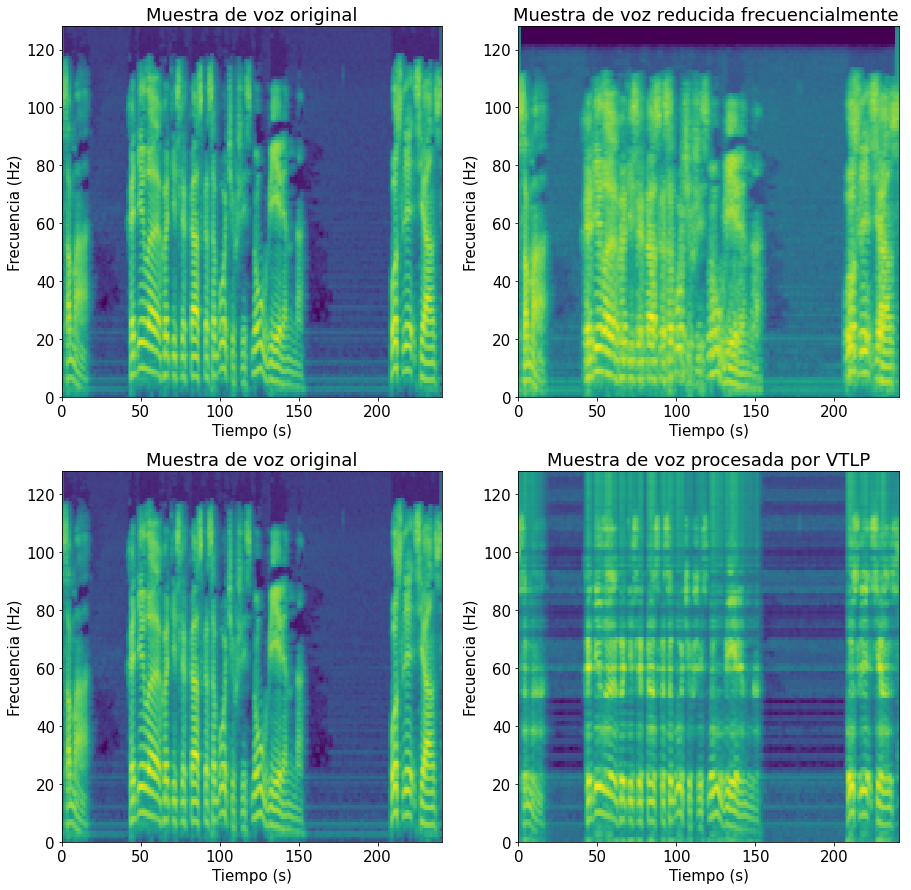
\includegraphics[scale=0.5]{imagenes/vtlp.png}
    \caption{Espectro de una voz modificada frecuencialmente, y mediante una transformación VTLP.}
    \label{fig:vtlp}
\end{figure}

\subsubsection{Algoritmo de Griffin-Lim}
El algoritmo de Griffin-Lim (ALG)\cite{griffin} es un método de reconstrucción de fase para señales de las que únicamente se tiene su componente de magnitud. El método de estimación de fase consiste de los siguientes pasos:

\begin{itemize}
    \item 1. Inicializar la fase aleatoriamente como ruido uniforme.
    \item 2. Realizar la transformada inversa de Fourier (inverse short-time Fourier transform, ISTFT).
    \item 3. Realizar la transformada de fourier (STFT) sobre la señal temporal obtenida. Esto deriva mínima información de fase de la señal temporal.
    \item 4. Reemplazar la magnitud obtenida por la STFT realizada por la magnitud de la señal original. Esto mantiene intacta la información de magnitud de la señal en el espectro, y agrega la minima información de fase de la señal que se deriva de la redundancia de la STFT.
    \item 5. Iterar los pasos 2-5 hasta obtener un resultado satisfactorio.
\end{itemize}
Iteración a iteración la información de fase resultara más pertinente a la componente de magnitud, dato original de la señal en el espectro. Muchos modelos de vocoder ignoran o tienen problemas para modelar la fase de una voz sintetizada. Este algoritmo puede ayudar a recrear en parte los artefactos característicos de algunos sistemas TTS.

\subsection{Vectorización de hablantes (speaker embeddings)}

La extracción de un descriptor numérico de cada audio a evaluar es un proceso necesario para el posterior entrenamiento de la red neuronal que se encargará de calificar cada modelo TTS. Los vectores de hablantes, (Speaker Embeddings) permiten extraer información critica de cada locutor a partir de una representación sonora del mismo, obteniendo un único descriptor capaz de codificar identidad de hablante, genero, velocidad del habla y contenido semántico del texto \cite{SpeakerEmbedding}. El proceso de extracción y la información codificada varía de implementación a implementación.

Los X-Vectors \cite{xvectors}, consisten en una representación vectorizada de cada hablante que aprovecha el uso de técnicas de DA. La representación resultante ha sido útil para mejorar la eficiencia de sistemas de reconocimiento de locutores. Una implementación de la red neuronal que extrae este tipo de descriptor se encuentra disponible en el Kaldi toolkit \cite{kaldi}.

Por otro lado HuBERT \cite{hubert} presenta una metodología auto-supervisada para extraer speaker embeddings. Existen tres problemas principales a la hora de generar este tipo de representaciones a partir de audios de una manera auto-supervisada, es decir, utilizando una base de datos no etiquetada: (1) existen más de una unidad sonora dentro de cada audio a procesar, (2) no existe un vocabulario o léxico de sonidos posibles en la etapa de pre-entrenamiento, y (3) la unidad sonora no tiene una segmentación explicita. Hubert presenta una implementación novedosa para la extracción auto-supervisada de speaker embeddings. Concretamente, el modelo aprende a agrupar (clustering) distintas unidades sonoras, enmascarando parte de la información, similar a la metodología planteada por \textbf{BERT}. La función de perdida se aplica únicamente sobre las regiones enmascaradas, forzando al modelo a aprender representaciones de alto nivel de la parte desenmascarada de la unidad sonora, para poder inferir correctamente respecto de como clasificar las regiones enmascaradas. Hubert extrae tanto información acústica, como lingüística como parte de su proceso de vectorización.

\newpage
\section{ESTADO DEL ARTE}
Determinar la calidad del habla sintetizada es una problemática que atraviesa distintas áreas y tecnologías: sistemas de texto a voz (TTS), mejora del habla (Speech Enhancement), y conversión de la voz (Voice Conversion) entre otros. Para el desarrollo de estos tipos de sistemas, donde las características de la señal de salida deben ser evaluadas repetidamente, surge la necesidad de utilizar modelos de calidad automáticos basados en criterios matemáticos y psicoacústicos para poder aproximar la apreciación subjetiva humana que se obtendría, por ejemplo, con un test MOS. El estado del arte de estas técnicas esta conformado por los siguientes sistemas:

%La Distancia Cepstral de Mel (MCD por sus siglas en inglés) \cite{melcepstral} es comúnmente %utilizada para medir la calidad del habla en la tarea de conversión de voz. MCD mide la %distorsión de distintos rasgos acústicos de una señal, sin embargo, los mismos no siempre se %ven correlacionados con la percepción humana.


\subsection{PESQ y POLQA}
Dentro del campo del speech enhancement, el PESQ \cite{pesq} (Perceptual Evaluation of Speech Quality o, evaluación percibida de calidad del habla), ITU T P.862, consiste en una evaluación intrusiva para cuantificar la calidad del habla. Es un algoritmo Full Reference (FR, o referencia completa), lo que quiere decir que para realizar una evaluación sobre un sistema requiere de la señal de entrada y de salida del mismo.  Su funcionamiento parte de un modelo psicoacústico, refinado empíricamente, que estima un valor MOS comparando la referencia original con la salida degradada del modelo, usando distancias paramétricas entre ambas señales. Al comparar la señal original y la señal degradada, las alinea en tiempo y normaliza en amplitud, por lo que no tiene en cuenta los efectos de distorsión temporal y de atenuación de la señal. Sin embargo, en muchos casos, para sistemas de TTS, no contamos con las señales originales utilizadas para entrenar una red neuronal (voz original), por lo que no se puede depender de algoritmos de este tipo.

En 2011, POLQA (Perceptual Objective Listening Quality Analysis)\cite{polqa}, ITU-T P.863, fue desarrollado como sucesor a PESQ. Este algoritmo compara muestra a muestra una señal degradada por un sistema, contra un señal original tomada como entrada de dicho sistema. Se analizan ambas señales en es dominio frecuencial, en distintas bandas criticas. Las diferencias encontradas  en cada banda son consideradas distorsiones, que luego son consideradas a la hora de asignar una puntuación tipo-MOS en una escala de 1-5. El aporte más relevante de este algoritmo es su modelo perceptivo, que toma en consideración ciertos factores humanos (\textit{Idealización}) de las tareas de categorización que se realizan durante tests MOS.

\subsection{ViSQOL}
ViSQOL (Virtual Speech Quality Objective Listener o, calidad del habla objetiva virtual) \cite{visqol}, fue desarrollado para emular la percepción humana sobre la calidad del habla. Evalúa una distancia calculada sobre un \textbf{neurograma}, análogo a un espectrograma, pero cuya intensidad (variable asignada al color del gráfico) está referida a la actividad neuronal. Nuevamente se trata de un algoritmo FR. Una comparación con las métricas desarrolladas por ITU, PESQ y POLQA, se realizó teniendo en cuenta la capacidad de cada algoritmo de detectar distintos tipos de transformaciones, incluyendo el añadido de distintos tipos de ruido de fondo, filtrado de señal, mejora del habla y variación de relación señal a ruido.

Los resultados de la investigación demostraron que ViSQOL y POLQA tienen un desempeño comparable, ambos superando el algoritmo PESQ.


\subsection{MOSNet}
Desarrollado para asistir en las tareas de evaluación de conversión de voz, MOSNet\cite{mosnet} es un predictor de valores MOS. El método propuesto consiste en entrenar una red neuronal sobre una base de datos construida a partir de evaluaciones de escucha realizadas durante el Voice Conversion Challenge 2018 (VCC). Para modelar la percepción humana tres diferentes arquitecturas son puestas a prueba y comparadas a lo largo de la investigación conducida por Chen-Chou, et al. 

El primer modelo, basado en una red convolucional concatenada a una capa completamente conectada, fue derivado del trabajo previo desarrollado por Yoshimura et al. \cite{yoshimura}. Las capas convolucionales fueron configuradas empíricamente para segmentar el discurso evaluado en secciones de 400 ms a modo de capturar información temporal más corta. El segundo modelo consiste en una red BLSTM (Bidirectional Long Short-Term Memory) previamente implementada en el paper Quality-Net \cite{qualitynet}, posee la habilidad de integrar la información de dependencias en el tiempo y de características secuenciales propias de una voz humana. Finalmente el tercer modelo es diseñado como una combinación de los dos previamente mencionados. 
Para cada arquitectura propuesta, el entrenamiento se realiza sobre características espectrales extraídas del VCC, con los puntajes MOS de dicha competencia como la solución objetivo. 
Los resultados indican una correlación alta entre los puntajes MOS derivados de los modelos entrenados, y los obtenidos por medio de pruebas subjetivas.

 \subsection{NISQA}
En 2021, Mittag y Moller \cite{mittag} presentaron un evaluador de naturalidad del habla sintetizada, basada en una red neuronal CNN-LSTM obteniendo resultados satisfactorios para oraciones, con pequeñas limitaciones cuando el espectro de la onda resultante se ve acotado. 
La base de datos utilizada en el entrenamiento esta compuesta de 16 fuentes distintas extraídas de distintas competencias realizadas de forma online, divididas en 12 idiomas distintos, para desarrollar una red neuronal capaz de procesar distintos lenguajes.
Una implementación abierta del código desarrollado por esta investigación se encuentra disponible. La misma permite ser re-entrenada con una nueva base de datos.

\subsection{Sinopsis de las distintas metricas de calidad objetiva presentadas}

En la Tabla \eqref{tab:ea}, se presenta una comparación entre las distintas arquitecturas discutidas en esta sección.

\begin{table}[h]
\centering
\caption{Sinopsis de las distintos modelos de calidad propuestos para predecir la preferencia humana}
\label{tab:ea}
\begin{tabular}{llll}
\textbf{Año} & \textbf{Referenica} & \textbf{Arquitectura}                                                                 & \textbf{Comentarios}                                                                                                       \\ \hline
2001         & PESQ                & Comparación intrusiva                                                                 & \begin{tabular}[c]{@{}l@{}}Primer metodología automatizada \\ adoptada por ITU\end{tabular}                                \\
2011         & POLQA               & \begin{tabular}[c]{@{}l@{}}Comparación intrusiva con\\ modelo perceptivo\end{tabular} & \begin{tabular}[c]{@{}l@{}}Sucesor de PESQ desarrollado \\ por ITU\end{tabular}                                            \\
2015         & VISQOL              & \begin{tabular}[c]{@{}l@{}}Comparación intrusiva con\\ modelo perceptivo\end{tabular} & \begin{tabular}[c]{@{}l@{}}Introducción del Neurograma \\ como modelo perceptivo\end{tabular}                              \\
2021         & MOSNet              & CNN-BLSTM                                                                             & \begin{tabular}[c]{@{}l@{}}Red neuronal entrenada sobre resultados\\ de encuestas tipo MOS de naturalidad\end{tabular}     \\
2021         & NISQA               & CNN‐LSTM                                                                              & \begin{tabular}[c]{@{}l@{}}También calcula otros parámetros \\ acústicos (ruido, distorsión y discontinuidad)\end{tabular}
\end{tabular}
\end{table}
\newpage
\newpage
\section{METODOLOGÍA}
\subsection{Obtención de datos}
Para poder entrenar un red neuronal capaz de predecir el resultado de un test tipo MOS realizado sobre un sistema de texto a voz, se necesita generar una base de datos con los resultados de un gran numero de algoritmos de síntesis vocal, acompañados de una etiqueta que represente su puntuación final obtenida de una prueba MOS. También se puede incluir en esa base de datos, ejemplos de voces humanas reales, y señales de voz sintetizadas, procesadas digitalmente.

Con el objetivo de generar esta robusta base de datos, en primera instancia se recolectaron ejemplos de un gran numero de sistemas de generación de voz humana disponibles. Los ejemplos a sintetizar fueron tomados de la lista de frases que forman parte del cuerpo de la base de datos de openSLR \cite{opensrl}: una base de datos generada por un equipo de investigación de Google, con el fin de entrenar sistemas de TTS y de ASR para idiomas de bajos recursos. Las lista completa de frases utilizadas son incluidas en el Anexo I.

En la Tabla \eqref{tab:dataset} se detallan los sistemas de texto a voz utilizados en la generación de la base de datos. Todos los ejemplos fueron sintetizados en castellano. El código de región exhibido en la tabla esta basado en el estándar ISO 639-1 para determinar la región de la voz sintetizada.

La base de datos incluye distintas voces sintetizadas con servicios profesionales de síntesis como Amazon Polly, Microsoft Azure, Speechello y Neurasound, sistemas concatenativos como Loquendo y la implementación TTS de Thomas Dewitte, servicios experimentales basados en Fastpich, y voces humanas reales pertenecientes al banco de voces OpenSRL.


\begin{table}[H]
\centering
\caption{Composición de la base de datos generada. Código de región de acuerdo a ISO 639-1.}
\label{tab:dataset}
\begin{tabular}{@{}ccccc@{}}
\hline
                                                                        & \textbf{Descripción}                                                          & \textbf{Región}                                                          & \textbf{Cant. de voces} \\ \hline
\textbf{\begin{tabular}[c]{@{}c@{}}Amazon \\ Polly\end{tabular}}        & Implementación privada                                                        & \begin{tabular}[c]{@{}c@{}}es-us/es-mx\\ /es\end{tabular}                & 8                       \\ \hline
\textbf{\begin{tabular}[c]{@{}c@{}}Microsoft \\ Azure\end{tabular}}     & Implementación privada                                                        & \begin{tabular}[c]{@{}c@{}}es-ar/es-bo\\ /es/es-mx\end{tabular}          & 8                       \\ \hline
                                                                        & Implementación privada (I.A.)                                                 & es-us/es-mx                                                              & 2                       \\
\multirow{-2}{*}{\textbf{Speechello}}                                   & Implementación privada                                                        & \begin{tabular}[c]{@{}c@{}}es-us/es-mx\\ /es\end{tabular}                & 5                       \\ \hline
\textbf{Neurasound}                                                     & Implementación privada                                                        & \begin{tabular}[c]{@{}c@{}}es-ar/es-cl/es-bo/\\ es-pe/es-pr\end{tabular} & 14                      \\ \hline
\textbf{Loquendo}                                & Sistema concatenativo                                                         & es                                                                       & 1                       \\ \hline
\textbf{\begin{tabular}[c]{@{}c@{}}text-to-\\ speech\end{tabular}}      & Librería de Python                                                            & es                                                                       & 1                       \\ \hline
\textbf{\begin{tabular}[c]{@{}c@{}}Fastpitch - \\ HiFiGan\end{tabular}} & \begin{tabular}[c]{@{}c@{}}Implementación con \\ transformadores\end{tabular} & es-ar                                                                    & 4                       \\ \hline
\textbf{DC-TTS}                                                         & Red convolucional                                                             & es-ar                                                                    & 7                       \\ \hline
\multicolumn{1}{l}{\textbf{TacoTron2}}                                  & Modelo secuencial                                                             & es                                                                       & 1                       \\ \hline
\textbf{OpenSRL}                                                        & Grabaciones de personas                                                       & es-ar                                                                    & 48                      \\ \hline
\end{tabular}
\end{table}

Esta base de datos inicial fue limpiada, transformada  y reducida durante el diseño de la prueba subjetiva, como será expuesto en la sección 4.3.


\subsection{Expansión artificial de datos}

Con el objetivo de variar los tipos de voces obtenidos en la sección previa, se llevo a cabo un proceso de expansión artificial de datos basada en distintas técnicas de procesamiento digital. Las mismas son detalladas a continuación:
\begin{itemize}
    \item \textbf{Alteración de largo tracto vocal (VTLP)}: 300 ejemplos de voces sintetizadas fueron procesados por este algroritmo, la implementación utilizada y el factor de deformación de VTLP (elegido aleatoriamente entre 0,9 y 1,1 para cada ejemplo) se basaron en recomendaciones detalladas por Jaitly et al. \cite{vtlp}.
            
    \item Alteración de fase (Algoritmo de Griffin-Lim): 500 ejemplos de voces reales y 100 ejemplos de voces sintetizadas fueron procesadas por este algoritmo de acuerdo al procedimiento especificado en la sección 2.3.2. 
    
\end{itemize}{}

\subsection{Diseño de la prueba subjetiva}

El diseño de la prueba subjetiva se basa en las especificaciones provistas por las recomendaciones del estándar ITU-T Rec. P.807. Todos los sujetos encuestados cumplieron con la condición de ser normo-oyentes.

El test consiste en la evaluación subjetiva de una serie de audios cortos que contienen distintas voces (2 a 6 segundos de duración). La duración total del test es de aproximadamente 8 minutos. Los ejemplo deben ser evaluados en una escala de tipo Likert de 5 puntos. La cantidad máxima de audios que un sujeto puede evaluar es de 50. El propósito de la encuesta subjetiva es el de etiquetar los audios recolectados previamente, con una puntuación. La cantidad de etiquetas necesarias está determinadas por el entrenamiento de la red neuronal que se desarrollará a posteriori. Un precedente útil se puede tomar del trabajo de Deja et al.[13] en el cual se llevó a cabo una metodología similar. Sujeto a la cantidad de audios que evalúe cada persona, en principio son necesarios alrededor de 100 sujetos de prueba, asumiendo que cada sujeto de prueba evalúe alrededor de 50 audios.

Una síntesis de las instrucciones presentadas a los participantes de la encuesta es provista a continuación:

\large{\textbf{Instrucciones}}

\normalsize

A continuación vas a escuchar una serie de distintos tipos de voces generados por computadoras. El propósito de este test es evaluar la calidad de cada archivo, para poder subsecuentemente utilizar esa información en un sistema de evaluación automático de voces sintetizadas.

Para cada ejemplo se deberá proveer una calificación de acuerdo a la siguiente escala. (Escala MOS para la naturalidad de una voz, Tabla \eqref{tab:instrucciones})

\begin{table}[H]
\centering
\caption{Escala MOS para la naturalidad de una voz}
\label{tab:instrucciones}
\begin{tabular}{cccll}
\textbf{Puntaje} & \textbf{Calidad del habla} & \textbf{Naturalidad}                    &  &  \\ \cline{1-3}
5                & Excelente                  & Completamente natural                   &  &  \\
4                & Buena                      & Bastante natural                        &  &  \\
3                & Aceptable                  & Natural y antinatural en partes iguales &  &  \\
2                & Mediocre                   & Bastante antinatural                    &  &  \\
1                & Mala                       & Completamente antinatural               &  & 
\end{tabular}
\end{table}

Los siguientes ejemplos ilustran el significado de cada puntaje. Sin embargo para realizar la prueba es importante tener en cuenta que se escucharan otros tipos de voces muy distintas, con distorsiones o artefactos no presentes previamente. Por lo tanto, estos ejemplos no cubren la totalidad de las posibilidades  que pueden esperar escuchar.

\large{\textbf{Ejemplos}}

\normalsize

El siguiente ejemplo presenta una voz humana y tiene un puntaje de referencia de 5.0

\begin{figure}[H]
    \centering
    
\includegraphics[scale=0.02]{imagenes/ale.jpg}
\end{figure}

El siguiente ejemplo presenta una voz sintetizada, puntaje de referencia de 4.0

\begin{figure}[H]
    \centering
    
\includegraphics[scale=0.02]{imagenes/ale.jpg}
\end{figure}

El siguiente ejemplo presenta una voz sintetizada, puntaje de referencia de 3.0

\begin{figure}[H]
    \centering
    
\includegraphics[scale=0.02]{imagenes/ale.jpg}
\end{figure}

El siguiente ejemplo presenta una voz sintetizada, puntaje de referencia de 2.0

\begin{figure}[H]
    \centering
    
\includegraphics[scale=0.02]{imagenes/ale.jpg}
\end{figure}

El siguiente ejemplo presenta una voz sintetizada, puntaje de referencia de 1.0

\begin{figure}[H]
    \centering
    
\includegraphics[scale=0.02]{imagenes/ale.jpg}
\end{figure}

Tener en cuenta que la calidad de los ejemplos que deberán clasificar puede ser distinta a la escuchada en estos ejemplos.


\subsubsection{Selección de respuestas validas}
Con el fin de descartar respuestas atípicas, se toman ciertos criterios para considerar validos los resultados de una prueba subjetiva:
\begin{itemize}
    \item Para cada ejemplo que se debe calificar, se tiene previamente un valor estimativo de la calidad esperada, extraído de encuestas previas y análisis objetivos. Por lo tanto si un candidato responde azarosamente, o simplemente deriva un criterio de calificación incorrecto por falta de claridad en las instrucciones,  es posible identificar y descartar sus respuestas.
    \item Se mide el tiempo de respuesta de cada estimulo. Se descartan los resultados que hayan sido entregados en un tiempo menor a un cierto umbral.
    \item Se toma los ejemplos a calificar de voces humanas reales como un “ancla", símil al concepto presente en otros tests subjetivos como el MuSHRA.
\end{itemize}

\subsubsection{Redistribución de audios a clasificar}

Para prevenir el sesgo de “ecualización de rango", los ejemplos provistos a los sujetos de prueba deben seguir una distribución uniforme respecto del rango de calidad total MOS definido para la naturalidad de la voz. La distribución de la base de datos debe ser perpetuamente balanceada en la medida que se obtienen resultados de distintas encuestas para asegurar la minimización de este sesgo.

Se llevó a cabo una prueba piloto de la evaluación propuesta que involucro a 5 participantes que calificaron 50 audios cada uno. Con los resultados obtenidos, se determinó un leve desbalanceo en en la calidad de los ejemplos sintetizados. En base a esto, se redefinió la base de datos obtenida previamente, para incluir más ejemplos de calidad estimada en el rango de 4,0 a 5,0. 


\subsection{Sistema de predicción de MOS}

\subsubsection{Funcionamiento general}
El funcionamiento del modelo de predicción cuenta de 3 etapas fundamentales: 1) Extractor de espectrograma de Mel y segmentación, 2) Extracción de características acústicas por franja, y 3) Extracción de características temporales. En la Figura \eqref{fig:fgeneral} se presenta un diagrama de la arquitectura implementada, que consiste de una modificación del modelo propuesto en \cite{qualityEst}.

\begin{figure}[h]
    \centering
    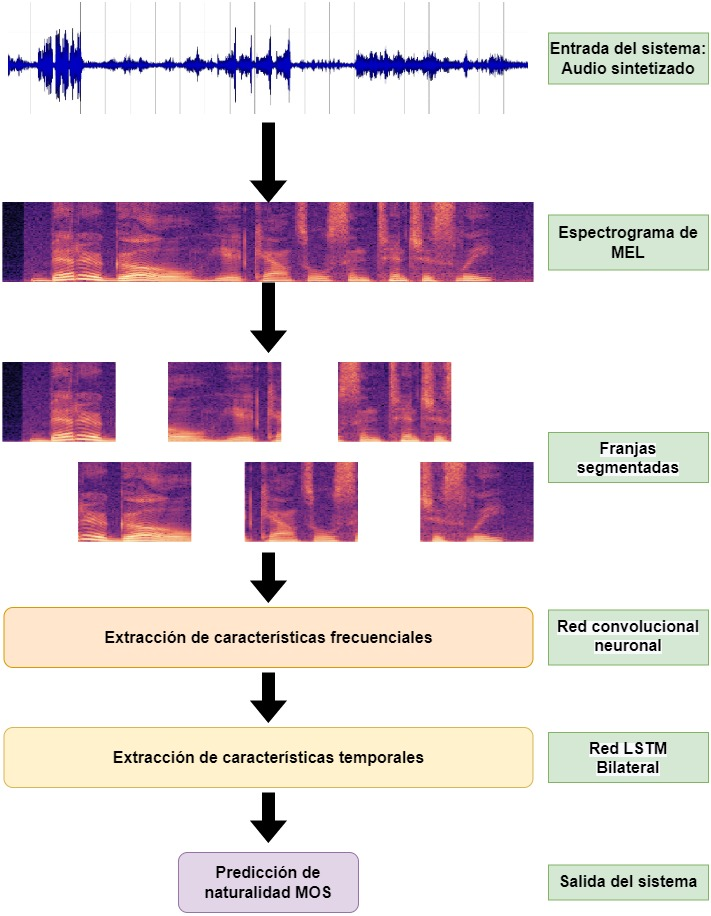
\includegraphics[scale=.45]{imagenes/funcionamiento_general.jpg}
    \caption{ Funcionamiento general del modelo de predicción de naturalidad MOS.}
    \label{fig:fgeneral}
\end{figure}

En primer lugar se extraen espectrogramas de Mel del audio a evaluar, separados en distintos segmentos con un cierto grado de solapamiento. Luego dichos segmentos son tomados como entrada de una red neuronal convolucional que extrae características útiles para predecir calidad sonora. Estas características se entregan a una red bilateral de larga-corta duración (BLSTM) que modela las dependencias temporales propias del discurso humano. La ultima capa completamente conectada de este segmento del modelo tiene como salida la predicción de naturalidad MOS.

\subsubsection{Segmentación en espectrogramas de MEL}
La entrada de la red neuronal convolucional toma espectrogramas de Mel generados a partir de una FFT con un tamaño de ventana de 20 ms y salto de 10 ms. El ancho de cada segmento es de 15, lo que equivale a 150 ms, y la altura es de 48 (48 x 15). La frecuencia máxima de análisis es de 20 kHz (muchos de los audios en el dataset tienen frecuencias de muestreo distintas). El tamaño de salto entre cada segmento es de 4 (40 ms), dando un cierto solapamiento de segmento a segmento. 

\subsubsection{Red CNN-BiLSTM}
Esta sección del modelo esta basado en la red siamés propuesta en \cite{qualityEst}. En la Figura \eqref{fig:cnn} se ofrece un diagrama para representar las distintas capas de este segmento del algoritmo de predicción. 

\begin{figure}[h]
    \centering
    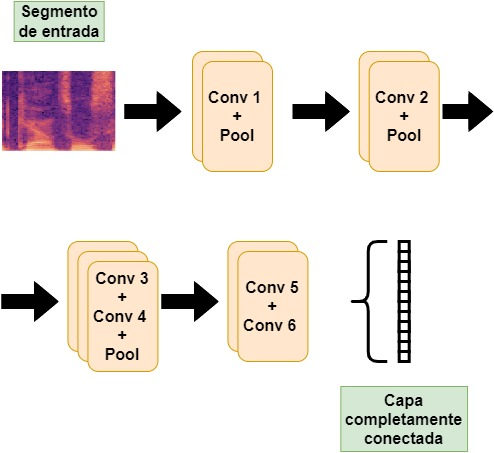
\includegraphics[scale=.45]{imagenes/cnn.jpg}
    \caption{ Arquitectura de la red neuronal convolucional. Cada capa esta acompañada por una activación de tipo ReLU.}
    \label{fig:cnn}
\end{figure}




La red esta tiene 6 capas convolucionales concatenadas, formadas por filtros de distintos tamaños como se puede observar en la Tabla \ref{tab:cnn}, donde N se corresponde con el numero de segmentos extraídos en la etapa previa, que depende de la duración del audio analizado. La salida de cada capa atraviesa una activación de tipo ReLU.

\begin{table}[]
\centering
\caption{Arquitectura de la red neuronal convolucional}
\label{tab:cnn}
\begin{tabular}{lllll}
\textbf{Capa}      & \textbf{Dimensión} &  &  &  \\ \cline{1-2}
Entrada            & Nx1x48x15          &  &  &  \\ \cline{1-2}
Conv1              & Nx16x48x15         &  &  &  \\
Pool               & Nx16x24x8          &  &  &  \\ \cline{1-2}
Conv2              & Nx32x24x8          &  &  &  \\
Pool-Perdida(20\%)  & Nx32x12x4          &  &  &  \\ \cline{1-2}
Conv3              & Nx64x12x4          &  &  &  \\
Conv4              & Nx64x12x4          &  &  &  \\
Pool-Perdida(20\%)  & Nx64x6x2           &  &  &  \\ \cline{1-2}
Conv5-Perdida(20\%) & Nx64x6x2           &  &  &  \\
Conv6              & Nx64x6x2           &  &  &  \\ \cline{1-2}
FC                 & Nx20               &  &  & 
\end{tabular}
\end{table}

La salida de esta etapa es utilizada como la entrada de una red de larga-corta duración bidireccional, de 1 sola capa con 128 unidades escondidas que se encarga de modelar las dependencias temporales de la señal y estimar finalmente la naturalidad del habla.

\subsubsection{Entrenamiento y detalle de la implementación}
El entrenamiento partió de pesos pre-entrenados con el NISQA Corpus \cite{nisqacorpus} una base de datos de audios en ingles evaluados subjetivamente por un gran numero de participantes. El ajuste fino de la red final se realizo sobre ese modelo, dividendo los resultados obtenidos de la encuesta subjetiva realizada en 80\% para el entrenamiento, y 20\% para la validación. 

El código necesario se implemento en el lenguaje de programación Python, sobre la biblioteca de DNN PyTorch y se encuentra disponible de en linea, en un repositorio \cite{repogit}. La velocidad de aprendizaje fue fijada en 0,001, se utilizo el optimizador Adam y se eligió la función de perdida consiente de sesgos, basándose en la metodología propuesta por \cite{biasloss}.

\subsection{Evaluación objetiva del sistema propuesto}

Para refinar el funcionamiento del modelo propuesto, (configuración de hiperparametros y características de la red propuesta), se analizan 2 métricas objetivas: correlación cruzada de Pearson ρ (PCC) y el error cuadrático medio (RMSE). {\color{red} \textit{En base a estas métricas se definirá el modelo final.}} \color{black} 

Para comparar el modelo propuesto con otras redes de predicción de calidad, ambas métricas propuestas son contrastadas con distintas soluciones del estado del arte: NISQA V1, NISQA V2 y ANIQUE+. La comparación se realiza sobre un subconjunto de ejemplos tomados de la base de datos desarrollada y evaluada subjetivamente a lo largo de este trabajo. Se evalúa el RSME y el PCC promedio sobre la totalidad del conjunto de audios, y también en distintas categorías como se presenta en la sección 5. 

En total, para cada modelo predictivo se evaluaron 200 audios, comparando el pronostico obtenido con el resultado subjetivo obtenido previamente. Se calcula RSME y PCC por estimulo, y seguidamente se obtiene un promedio de ambas métricas a nivel de cada sistema evaluado.


\newpage
\section{RESULTADOS Y ANÁLISIS}
\subsection{Resultados iniciales}

Se presentan los resultados iniciales en la Tabla \ref{tab:resultados}. El RMSE y ρ a nivel de sistema se calcularon para el modelo predictivo propuesto, y para la segunda iteración del software NISQA. En ambos casos, se procesaron y evaluaron audios juzgados bajo 2 condiciones:
\begin{itemize}
    \item RMSE y coeficiente de correlación ρ calculado sobre las encuestas realizadas previas a balancear la base de datos (250 ejemplos utilizados en el entrenamiento del modelo propuesto)
    \item RMSE y coeficiente de correlación ρ calculado sobre las encuestas realizadas posterior a balancear la base de datos (500 ejemplos utilizados en el entrenamiento del modelo propuesto)
    \item RMSE y coeficiente de correlación ρ calculado sobre las encuestas realizadas posterior a balancear la base de datos (750 ejemplos utilizados en el entrenamiento del modelo propuesto)
    
\end{itemize} 

\begin{table}[h]
\centering
\caption{Resultados iniciales obtenidos con 15\% de los audios de la base de datos evaluados}
\label{tab:resultados}

\begin{tabular}{ccccc}
                                                                                          & \multicolumn{2}{c}{\textbf{Modelo propuesto}} & \multicolumn{2}{c}{\textbf{NISQA V.2}} \\
                                                                                          & ρ                     & RSME                  & ρ                  & RSME              \\ \hline
\begin{tabular}[c]{@{}c@{}}Previo a \\ balancear el dataset\end{tabular}                  & 0,32                  & 2,63                  & 0,17               & 3,19              \\ \hline
\begin{tabular}[c]{@{}c@{}}Posterior a \\ balancear el dataset\end{tabular}               & 0,35                  & 1,63                  & 0,31               & 2,07              \\ \hline
\begin{tabular}[c]{@{}c@{}}Posterior a balancear \\ el dataset +250 ejemplos\end{tabular} & 0,49                  & 1,21                  & 0,24               & 2,04             
\end{tabular}
\end{table}


\subsection{Tiempo de procesamiento}

\subsection{Modelo final}

\newpage
\newpage
\section{DISCUSIÓN DE LOS RESULTADOS}
(\color{red}\textit{Discusión de los resultados iniciales de la entrega \textbf{Avance 4} del Taller de Tesis.})\color{black}

Los resultados iniciales obtenidos nos permiten inferir ciertas hipótesis que pueden resultar útiles a la hora de continuar el desarrollo del trabajo:

\begin{itemize}
    \item En primer lugar, como es de esperarse los resultados mejoran al incorporar más ejemplos de entrenamiento. Por ahora, la cantidad de datos recolectados son 10\% de la totalidad que se espera obtener para el entrenamiento del modelo final, por lo que se espera una mejora significativa de las métricas evaluadas en el futuro, simplemente por tener una base de datos más robusta.
    \item La segunda iteración de los resultados fueron calculados luego de balancear los estímulos de prueba. Es posible que parte de la mejora en el RMSE se deba a este ajuste de la encuesta realizada, por lo que se propone realizar un balanceo adicional antes de liberar la evaluación subjetiva al publico general para obtener el resto de las respuestas necesarias
    \item Si bien el modelo propuesto supero el desempeño de la red NISQA V.2, esto se debe en parte a que la red NISQA nunca había sido expuesta a audios en el idioma castellano en su entrenamiento. Al mismo tiempo, el modelo propuesto fue entrenado con audios que guardan cierta similitud a los que fueron usados en la evaluación (ambos subconjuntos de la misma base de datos), lo que puede aportar otro factor que beneficie a un modelo predictivo sobre el otro.
    \item Para futuras comparaciones es importante incluir otros modelos como NISQA V1 y ANIQUE+
    \item Es posible adoptar variaciones sobre la arquitectura propuesta, para poder refinar el sistema aún más. La mayoría de los cambios significativos son propios de la red neuronal convolucional.
\end{itemize}


\newpage
\newpage
\section{CONCLUSIONES}



\newpage
\section{TRABAJOS FUTUROS}
\color{red}
\textit{Al finalizar el desarrollo, de acuerdo a los resultados alcanzados, se podría evaluar el modelo realizado en otros idiomas para verificar su funcionamiento multilingüe. Otro posible desarrollo será obtener una base de datos más robusta, con un número de encuestados mayor, para re-entrenar y refinar el funcionamiento de la red neuronal. También se plantea la posibilidad de empaquetar el modelo para poder ser utilizado como una librería de Python disponible como código abierto, para facilitar su uso en producción de sistemas TTS.} \color{black}

\newpage
\section{Anexo I: Listado de frases utilizadas para sintetizar audios}

Para la caída del cabello, tengo un nuevo jabón

¿Qué color favorito es el más popular?

El pijama de rayas es azul

Las máquinas de escribir antiguas pueden ser muy caras.

Al circular menos automóviles en la ciudad se logra una mejor calidad del aire

¿A qué hora querés ir al cine?

Estoy destinada a triunfar

Tengo una junta de negocios con la firma de abogados, ¿se acuerda?

Para abrir los poros de la piel lo mejor es ir a un sauna, o tomar un baño de vapor

Para hacer esa receta necesitás fruta y alcohol

Quiero que me ayudes a elegir un regalo.

La obscuridad del pozo era obscena por naturaleza

Aquí doblamos a la derecha

Las tejas rojas del tejado no son de México, son de Texas

Estaba pensando en ir a acampar.

Lo podés pagar con la tarjeta verde de Visa

¿Cuáles son las principales diferencias?

¿Cuál es la estación de metro más cercana?

Si el cuerpo pide descanso hay que dárselo dicen los médicos

Mañana vaya abrigada, un gorro de lana y guantes es lo más recomendable

El viaje en avión es más rápido que en barco.

¿Quién subió el mejor video?

La pronunciación del francés es difícil

Me ayudas a plantar los naranjos

El Llano en Llamas es un clásico de Juan Rulfo

Quiero averiguar como se llama un director de cine

¿Cuándo sucedió la Primera Guerra Mundial?

Este personaje malverso una cantidad extraordinaria de fondos públicos

En las noticias de anoche, no vi que al presidente de Estados Unidos.

Las bocinas estas que te dije son enormes, ¿sabés que se puede hacer con ellas?

Es muy fácil usar las bicis de la ciudad, con tu tarjeta de crédito alquilas tu bici.

Mañana va a hacer mucho viento y habrá tormentas

El dictador Franco estuvo cuarenta años en el poder.

¿Quién subió el mejor video?

Te voy a mandar por whatsapp las especificaciones de los invitados

La calle está llena de hoyos

Tenés que denunciar inmediatamente el accidente para que lo cubra el seguro

Quiero un jabón para relajarme.

Necesito tu ayuda urgente.

¿Qué tan destruida quedó la ciudad de Nueva Orleans después del huracán Katrina?

Los hamsters comen zanahorias

En el salón de fiestas entran alrededor de mil quinientas personas

Hoy a la tarde saqué mi tarjeta para la bicicleta urbana

Ayudáme a encontrar un buen gimnasio pero que esté cerca de mi casa

No te entiendo nada

La granizada destruyó toda la plantación de lechuga

Quiero irme de vacaciones a Hawái pero no sé si el volcán esté activo.

Se hicieron versiones en todos los idiomas de esa canción

Voy a necesitar que lo pagués con la tarjeta roja

Te recomiendo que te llevés un buen libro o bajés una buena película

¿Queres que te recomiende algo en particular?

Además, no necesitás comprar una bicicleta, podés usar las de la ciudad.

No sé hablar malayo

¿Deseas avisar a tu familia que estás bien?

Te quiero pedir cincuenta bolsas de basura extra grandes y veinticinco carpas

¿Podés verificar si hay alguna estación de tren cerca del aeropuerto?

La piel es muy porosa

Del subte al museo son quince minutos

¿Hay algún video viral esta mañana?

Quiero ver una película pero que sea en una pantalla grande.

¿Querés aprender el idioma a nivel de negocios?

Te quiero pedir cincuenta bolsas de basura extra grandes y veinticinco carpas

¿Me ayudas a hacer los deberes?

Creo que se le disloco el hombro

El siguiente semestre quiero empezar a estudiar licenciatura en cine

Los atajos están más libres de circulación que nunca en los últimos tiempos

No entiendo nada

Me gustaría organizar unas charlas sobre mecanica industrial

Él sabe que con eso va a pasar a la historia.

La parte de las cataratas del Niágara que está del lado estadounidense es aburrida

Les recomiendo que escalen siete montañas de más de mil metros sobre el nivel del mar

Los champiñones silvestres son los más sabrosos

Corea del Norte logró lanzar un misil a una distancia de quinientos km por primera vez.

Últimamente he visto muchas bicicletas en la calle.

Últimamente he andado muy acelerada.

El caballo está amarrado

Tocar el xilófono es mi hobby favorito

¿Es un vuelo directo o hace escalas?

Quiero que me des tu opinión sobre la nueva obra de teatro.

¿Sabes de electricidad?, necesito cambiar un enchufe y no se como

Te voy a mandar una lista de los mejores exitos en español directo a tu celular.

Estoy acá con una amiga cocinando comida Tailandesa

Estoy aburrido con la música de mi teléfono, quiero que me recomiendes algo nuevo.

La película me llegó al corazón

Le recomiendo los Alpes Suizos

El Llano en Llamas es un clásico de Juan Rulfo

¿Podrías comprar por favor el disco y enviarselo a mi mamá?

Este libro nos muestra una teoría sobre la importancia del arte en el ámbito científico

La obra de teatro El Flautista fue un exito rotundo

Mas o menos ¿qué presupuesto está dispuesto a pagar?

Estoy buscando un restaurante de cocina tradicional

¿Me podés ayudar a coser un parche?

Los hamsters comen zanahorias

Tiene el tiempo contado

No entiendo nada

Quiero ver una película de comedia

Primero que nada vamos a hacer un ejercicio de respiración

Los hamsters comen zanahorias

La ciudad es bellísima y tan alegre


\onecolumn
\section{Anexo II: Código Implementado}
\newpage

\renewcommand\refname{BIBLIOGRAFÍA}
\begin{thebibliography}{20}

\import{sections/}{bib}

\end{thebibliography}
%\appendix
%\section{}
%123



\end{document}
